\documentclass[a4paper,titlepage]{article}
\usepackage[]{mcode}
\usepackage{natbib}
\usepackage{graphicx}
\usepackage{hyperref}
\usepackage{amsthm}
\usepackage{amsmath}
\usepackage[margin=2cm]{geometry}

\begin{document}

\begin{titlepage}
	\newcommand{\HRule}{\rule{\linewidth}{0.5mm}}
	\center

	%------------------------------------------------
	%   Logo
	%------------------------------------------------

	
\includegraphics[width=0.2\textwidth]{Crest.jpg}\\[1cm]

	%------------------------------------------------
	%	Headings
	%------------------------------------------------

	\textsc{\LARGE University of Exeter}\\[1.5cm]

	\textsc{\Large College of Engineering, Mathematics and Physical Sciences}\\[0.5cm]

	\textsc{\large ECM3735 - Group 8}\\[0.5cm]

	%------------------------------------------------
	%	Title
	%------------------------------------------------

	\HRule\\[0.4cm]

	{\huge\bfseries Finding the optimal strategy for the dice game `Pig'}\\[0.4cm]

	\HRule\\[1.5cm]

	%------------------------------------------------
	%	Authors
	%------------------------------------------------

	\LARGE\textit{Authors}\\
	\begin{minipage}{0.4\textwidth}
		\begin{flushleft}
			\large
			S. \textsc{Bayliss}\\
			A. \textsc{Dunford}\\
			E. \textsc{Morison}\\
			J. \textsc{Peet}\\
			L. \textsc{Sutton}
		\end{flushleft}
	\end{minipage}
	~
	\begin{minipage}{0.4\textwidth}
		\begin{flushright}
			\large
			C. \textsc{Crawford}\\
			R. \textsc{Jones}\\
			C. \textsc{Nash}\\
			A. \textsc{Smith}
			\vspace*{10pt§}
		\end{flushright}
	\end{minipage}

	\vfill\vfill
	\textit{Supervisor}\\
	Dr. B. \textsc{Cooper}

	%------------------------------------------------
	%	Date
	%------------------------------------------------

	\vfill\vfill\vfill

	{\large\today}
	\vfill

	%------------------------------------------------
	%	Abstract
	%------------------------------------------------

	\newpage
	\begin{abstract}
	\textit{Insert abstract here}
	\end{abstract}
\end{titlepage}

	%------------------------------------------------
	%	Contents
	%------------------------------------------------

\tableofcontents
\newpage

\section{Introduction}
\subsection{Aims and Objectives}
josh
\subsection{History of Pig}
\subsubsection{Basics of Pig}
The dice game `pig' is played by 2 people rolling a die. The number on the die signifies the points gained on that roll, which are collated in a sum total of points for the turn. These points can be banked to bring a players turn to an end. However, the points in this rolling total can be lost if the player rolls a $1$, this will also automatically bring their turn to an end. The aim of the game is to be the first player to have a banked total of points greater than or equal to $100$.
\\
\\
The probabilities of winning the game from any position can be simplified down into sets of linear equations. Suppose I have 2 strategies A and B. Consider that it is A's turn and we are in position ($i,j,k$) where $i$ is A's banked points, $j$ is B's banked points, and $k$ is A's sum total of points so far on this turn. Let $P_{ijk}$ denote the probability of A winning from the current position and $Q_{ijk}$ denote probability of B winning from the equivalent position (where $i$ then represents B's banked points etc.). Then, \begin{equation}\label{1.2.1.a}
p_{ijk} = \dfrac{1}{6} (1-Q_{ij0}) + \dfrac{1}{6}\sum^{6}_{r=2}P_{ijk+r}
\end{equation}
 if A rolls and
 \begin{equation}\label{1.2.1.b}
 p_{ijk} = 1-Q_{jik}
 \end{equation}
 if A banks their points.
\subsubsection{Nellers Work}
In \textit{Dice Games Properly Explained}, Reiner Knizia takes the view of each roll of the die in `pig' as a bet of not rolling a $1$. He viewed the best strategy as ``Whenever your accumulated points are less than 20, you should continue throwing, because the odds are in your favour.''\cite{knizia2010dice}. However, Todd W Neller stated ``\textit{risking points is not the same as risking the probability of winning.}''\cite{neller2004optimal}, from this Neller proceeded to find a more optimal solution for `pig' by taking the maximum of equation \ref{1.2.1.a} and equation \ref{1.2.1.b}. This was not possible however as he ended up with an equation of the form $x=$max$ (A_1 x+b_1,A_2 x+b_2)$ for which there is no known general method. As a result Neller implemented value iteration to calculate an accurate estimate for the probabilities at each position $(i,j,k)$ for both bank and roll. Figure \ref{figure1} shows the resulting optimal strategy where you should roll if you are below the surface of the graph and bank if above.

\begin{figure}
\centering
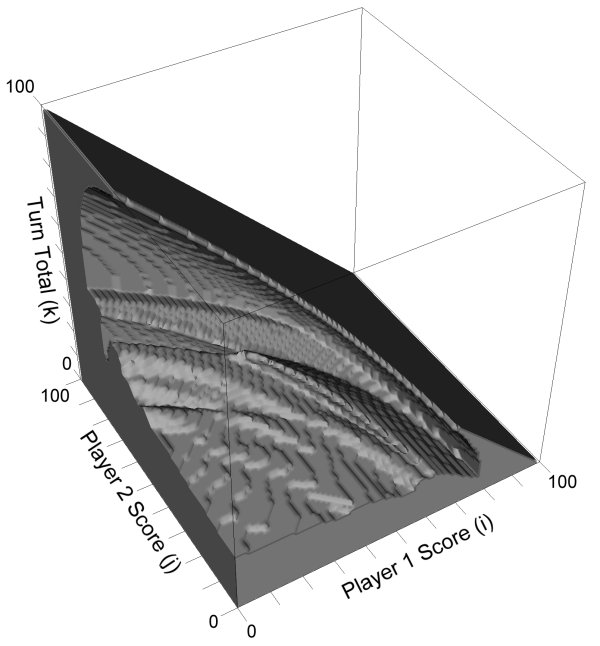
\includegraphics[width=0.5\textwidth]{neller_optimal_solution}
\caption{roll\slash hold boundary for the optimal Pig play policy (Neller)\label{figure1}}
\end{figure}
\begin{figure}
\centering
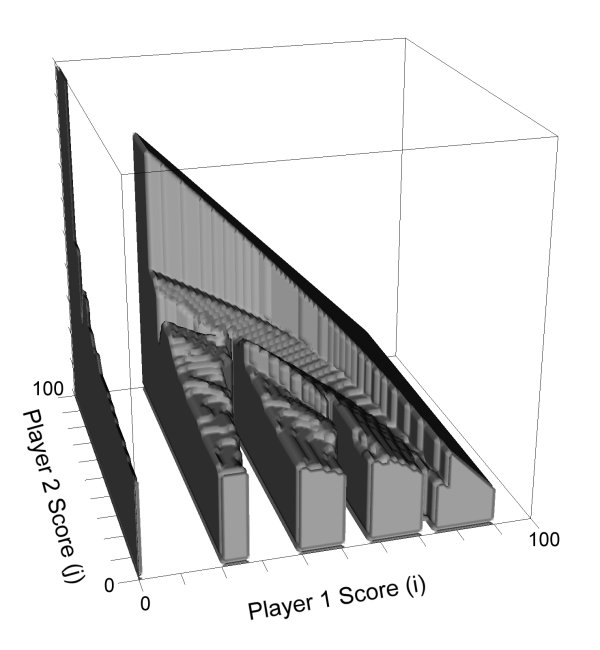
\includegraphics[width=0.5\textwidth]{neller_optimal_solution_2}
\caption{all of the states reachable by an optimal player (Neller)\label{figure2}}
\end{figure}

\subsection{Optimal Stratergy}
chris C
\subsection{Preliminary Findings}
chris N

% Playing the game together

\section{Methodology}
\subsection{Group Organisation}
Mia
\subsubsection{Meetings}
\subsubsection{Creation of Prject Plan}

\subsubsection{Similataneous Equations}

Anthony

% Outline how to solve for the probabilities by similitanious equations.

\subsection{Piglet}
Chris C

% Introduce Piglet, differnces from pig (how it is simpler)

% Important difference with gaining points (piglet adds 1 to socre but dice adds from 2)

\subsubsection{Hand Written notes}
Chris C

% Piglet to 2/3 with simple bank on strategies.

% Wrote out each similtaneous equations set and the matrix form.

\subsection{Coding}

% Required knowledge:
% - Similataneous equation sets
% - Matrix form of the sets

Once we had familisirised ourselves with the rules of the game, the equations, and
a few simple piglet examples, we moved to matlab.
The end goal is the make use of Matlab's computational power, to solve thousands of
similtaneous equations and find all the probabilites at each game state.
We can also make use of variable inputs to compare any strategy to another, and
even change the score needed to win and the dice probability.

Our first attempt at simply getting out ideas down as code was a very simplified
calculation of piglet. Although we coded in a dice probability variable that could be changed,
the code only worked for a dice flip, and when the variable was set to $\frac{1}{2}$.
It was also limited to taking in only Bank on strategies.
%Explain what Bank on strats are
We could however run to any winning score.

The way we got Matlab to solve the sets of similtanious equations was by turning them into
matrices of coefficients, variables and constants. $CX=D$ This was discussed before
and will be touched on again to talk about the layout of the matrices in the more general
refined code for pig.

By using the hand calculated simple piglet probabilities we could check to see if our
coded matrices were correct and fix any bugs. Once this was working we had our first
runnable code to get us going. We just had to generalise the code.
There were two steps to doing this; taking any strategy as an input, and having any
dice probability working in the code. The former was easier; an independent problem that we
made a function to do for us. The later was a little trickier but was a fundamental part
of building the matrices.

% Subsection on Strategies to matrices

% Subsection on coding matrices

...

Once we had done this, we had a generalised working code that could calculate the
probabilities of winning at any game state, for any two strategies, for any given
dice proability and to any winning score.

\subsubsection{Debugging of the code}

% Rhodri

% The layout of subsections needs to change but the subsection below on debuggin
% can come right after the last thing i wrote in "coding for pig" ( For Rhodri, from Ant <3 )

\subsection{Behavioural Economics}
Mia and Josh

\subsection{Statistical Testing}
eliot and sam
\subsubsection{Fair test}
\subsubsection{Theory of Hypothosis testing}
\subsubsection{Running of tests}


\section{Findings}
\subsection{Pig}
\subsubsection{Did we solve Pig}
{\tiny YES.}

\subsection{Behavioural Economics}
\subsubsection{Do players stick to their risk preference}
\subsubsection{Players Interactions}

\subsection{Statistical Testing}
\subsubsection{Non-transitivity}
\subsubsection{Testing against our optimal}
\subsubsection{Testing against Nellers optimal}


\section{Conclusions}
\subsection{Overall findings}
\subsection{Determination of human affects on the optimal stratergy}
\subsection{Comparison to Nellers stratergy}

\nocite{*}
\bibliographystyle{alpha}
\bibliography{Pig_bib}
\end{document}
